\documentclass[12pt,a4paper]{article}
\usepackage[warn]{mathtext}
\usepackage[utf8]{inputenc}
\usepackage[english,russian]{babel}
\usepackage{amsmath}
\usepackage{amssymb}
\usepackage{latexsym}
\usepackage{svg}
\usepackage{indentfirst}
\usepackage{pgfplots}
\pgfplotsset{compat=1.9}

\usepackage{listings}

\usepackage{color}

\definecolor{dkgreen}{rgb}{0,0.6,0}
\definecolor{gray}{rgb}{0.5,0.5,0.5}
\definecolor{mauve}{rgb}{0.58,0,0.82}

\lstset{ %
	language=C++,                % Язык программирования 
	numbers=left,                   % С какой стороны нумеровать
	stepnumber=1,                   % Шаг между линиями. Если 1, то будет пронумерована каждая строка
	frame=single,	
}
\usepackage[left=2cm,right=2cm,
top=2cm,bottom=2cm,bindingoffset=0cm]{geometry}

\usepackage{sverb}
\usepackage{graphicx}
\usepackage{pdfpages}
\usepackage[absolute,overlay]{textpos}

\numberwithin{equation}{section}

\begin{document}
	\begin{titlepage}
		\begin{textblock*}{13cm}(0cm,0cm)
			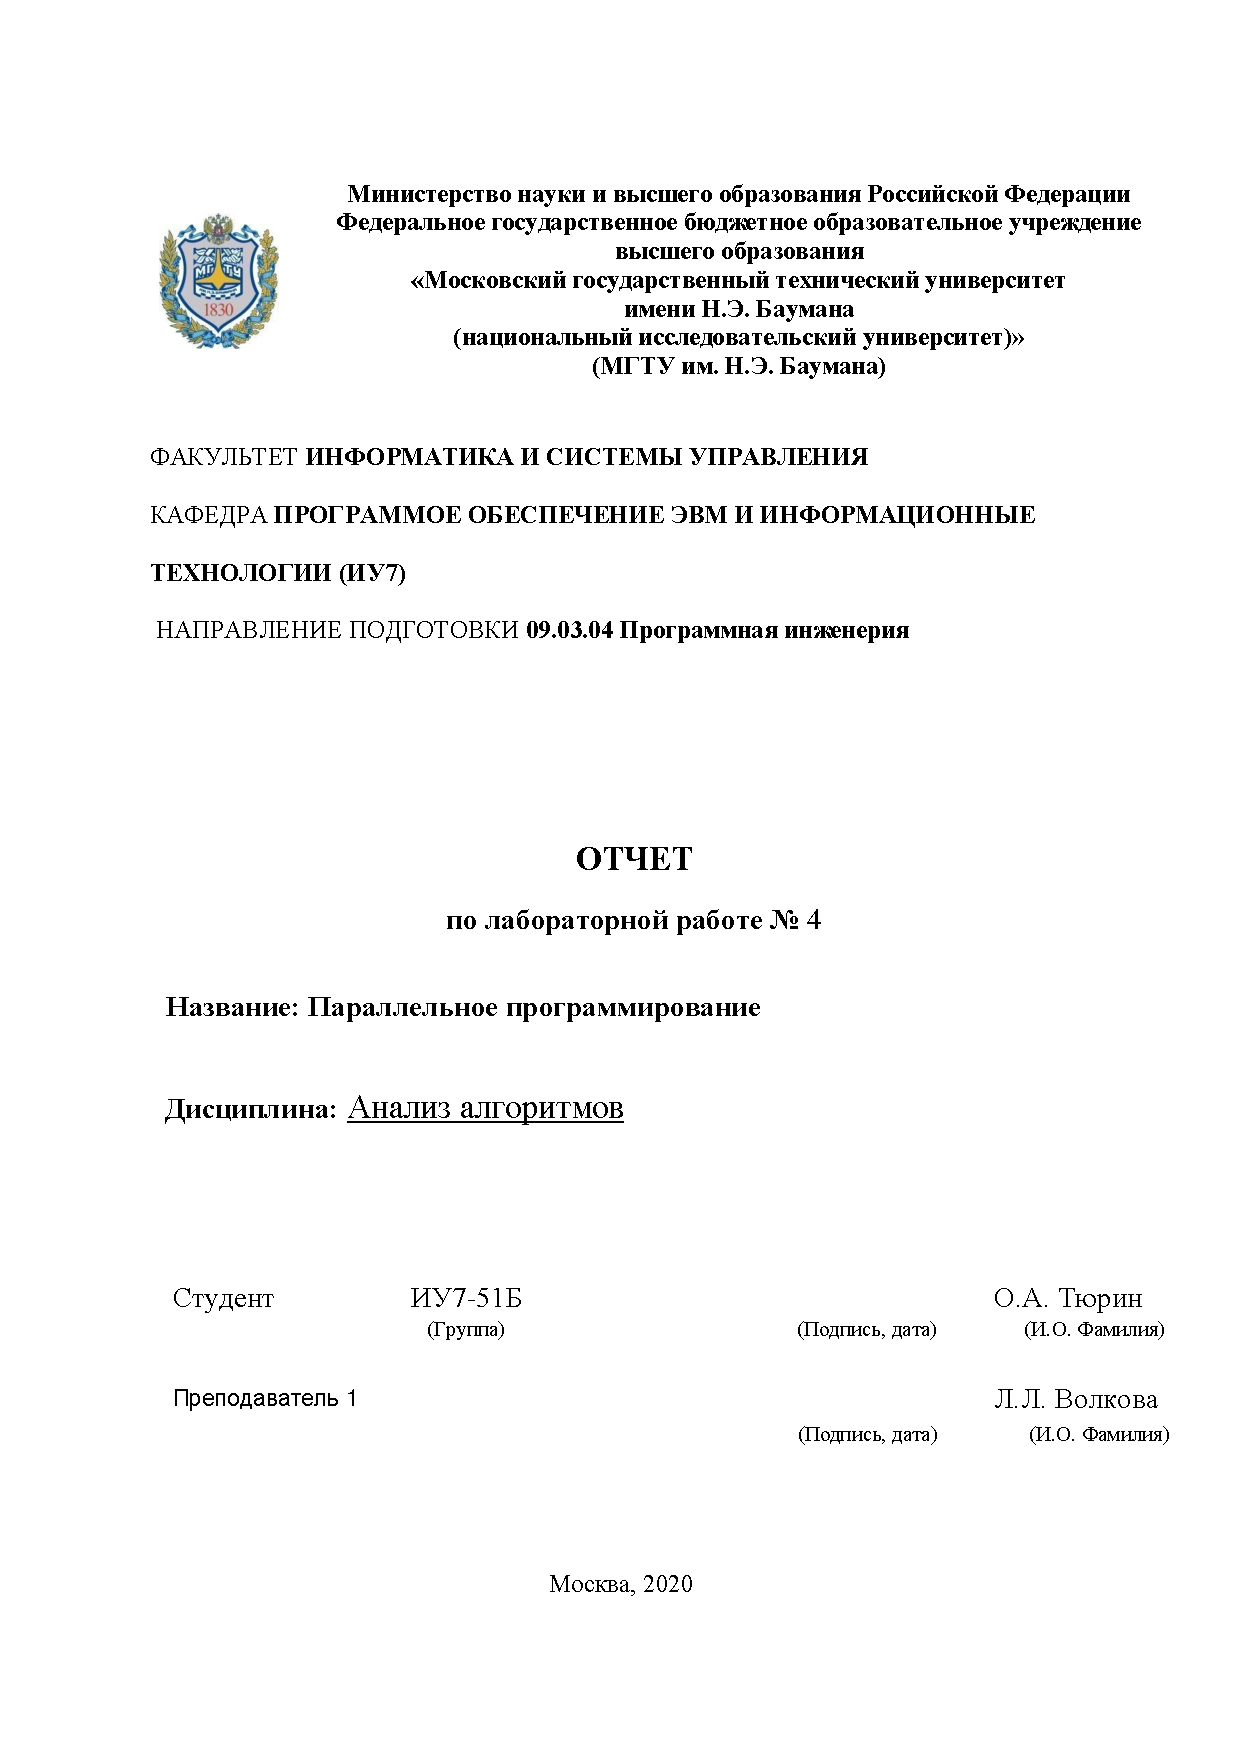
\includegraphics{reportTitle}
		\end{textblock*}
	\end{titlepage}
\hspace{0pt}
\clearpage
%	\begin{titlepage}
%		\centering
%		\Huge Лабораторная работа №1 по курсу \\\textbf{"Анализ алгоритмов"}\\
%		Тема: Расстояния Левенштейна и Дамерау-Левенштейна\\
%		\vspace{\baselineskip}
%		\Large Работу выполнил: Колосов Д.В ИУ7-52Б\\
%		Преподаватели: Волкова Л.Л, Строганов Ю.В.
%		\vfill
%		Москва, 2020 г.		
%	\end{titlepage}
\tableofcontents
\clearpage

\addcontentsline{toc}{section}{Введение}
%//////////////////////////////////////////////////////////////////
\section*{\Huge Введение}
Цель данной работы - изучение возможности параллельных вычислений и использование такого подхода на практике.

В даной лабораторной работе рассматривается простой алгоритм нахождения суммы элементов подмассива и его параллельная версия, представленная в двух вариантах.\\
Задачами данной лабораторной работы являются:\\
\begin{itemize}
	\item рассмотрение стандартного алгоритма подсчёта суммы элементов массива;
	\item проведение сравнительного анализа последовательного алгоритма подсчёта и двух его пареллельных реализаций;
	\item определение зависимости времени работы алгоритма от числа потоков исполнения и количества слов.
\end{itemize}

\clearpage

\section{Аналитическая часть}
В данном разделе будет расмотрена теоретическая часть алгоритма подсчёта количества вхождений каждого символа в наборе строк и теоретические основы параллельного программирования.

\subsection{Описание алгоритмов}
\qquad В данном разделе будут описан каждый исследуемый алгоритм.

\subsection{Стандартный алгоритм}
Пусть дана последовательность чисел, длина последовательности - n.\\
Для того, чтобы подсчитать сумму элементов каждого подмассива, необходимо создать дополнительную переменную, и массив, который имеет размерность n.

Далее необходимо проитерировать каждый подмассив, и подсчитать в нем сумму.\\
Пример:
\begin{center}
	numbers = \{\{1, 2, 3\}, \{4, 5, 6\}, \{7, 8, 9\}\}
\end{center}

Проходимся по каждому подмассиву, ищем сумму и записываем в результирующий вектор res.
\begin{center}
sum(\{1, 2, 3\}) = 6\\
res = \{6\}\\
sum(\{4, 5, 6\}) = 15\\
res = \{6, 15\}\\
sum(\{7, 8, 9\}) = 24\\
res = \{6, 15, 24\}\\
\end{center}

Сумма ищется следющим способом:\\
Пример:\\
Возьмем подмассив \{1, 2, 3\}\\
Объявлем переменную resuslt = 0, в которую будет записываться сумма подмассива.\\
Далее итерируемся по подмассиву, прибавляя к result текущий элемент.\\

Таким образом, в res хранится последовательность, означающая сумму чисел каждого подмассива исходного массива.

\subsection{Первая реализация паралелльного алгоритма}
Реализуем некую очередь, в которой каждый из потоков будет брать следующуй подмассив. Таким образом, как только поток освобождается - он берёт следующий подмассив из очереди.\\
Пример: \\
Пусть есть 2 потока и следующий список подмассивов:
\begin{center}
	numbers = \{\{1, 2, 3\}, \{4, 5, 6\}, \{7, 8, 9\}\}
\end{center}
Первый поток берёт на обработку подмассив \{1, 2, 3\} (обработка аналогична описанной в пункте выше). Второй поток в это время берёт на обработку подмассив \{4, 5, 6\}. Далее первый поток берёт на обработку подмассив  \{7, 8, 9\}. Выполнение алгоритма завершено. В данном алгоритме очень важно следить за корректным забором элементов из очереди, а также за корректном добавлении в результирующий массив.

\subsection{Вторая реализация паралелльного алгоритма}
Так как количество подмассивов заранее известно, то каждому из потоков можно выдать одинаковое количество подмассивов на обработку, поделив количество подмассивов на число потоков.\\
Пример: \\
Пусть есть 3 потока и следующий список строк:
\begin{center}
	numbers = \{\{1, 2, 3\}, \{4, 5, 6\}, \{7, 8, 9\}, \{\{1, 2, 4\}, \{5, 7, 9\}, \{6, 8, 4\}\}
\end{center}
Колчиство подмассивов - 6.\\
Количество потоков - 3.\\
Слеовательно, количество подмассивов на обработку для каждого потока - 2.\\
Для упрошения каждому из потоков можно давать на обработку те подмассивы, номера которых лежат между номером потока, умноженного на количество подмассивов, поделённое на количество потоков и номером следующего потока, умноженного на количество подмассивов, поделённое на количество потоков:
\begin{equation}
	start = \frac{threadID * arrQuantity}{threadsQuantity}\\
\end{equation}
\begin{equation}
	end = \frac{(threadID + 1) * arrQuantity}{threadsQuantity}\\
\end{equation}

\subsection{Параллельное программирование}
При использовании многопроцессорных вычислительных систем с общей памятью обычно предполагается, что имеющиеся в составе системы процессоры обладают равной производительностью, являются равноправными при доступе к общей памяти, и время доступа к памяти является одинаковым (при одновременном доступе нескольких процессоров к одному и тому же элементу памяти очередность и синхронизация доступа обеспечивается на аппаратном уровне). Многопроцессорные системы подобного типа обычно именуются симметричными мультипроцессорами (symmetric multiprocessors, SMP) \cite{litlink3}.\\

Обычный подход при организации вычислений для многопроцессорных вычислительных систем с общей памятью – создание новых параллельных методов на основе обычных
последовательных программ, в которых или автоматически компилятором, или непосредственно программистом выделяются участки независимых друг от друга вычислений. Возможности автоматического анализа программ для порождения параллельных вычислений достаточно ограничены, и второй подход является преобладающим.\\

Широко используемый подход состоит и в применении тех или иных библиотек, обеспечивающих определенный программный интерфейс (application programming interface,
API) для разработки параллельных программ. В рамках такого подхода наиболее известны Windows Thread API \cite{litlink1}. Однако первый способ применим только для ОС семейства
Microsoft Windows, а второй вариант API является достаточно трудоемким для использования и имеет низкоуровневый характер

\subsection {Организация взаимодействия параллельных потоков}
Потоки исполняются в общем адресном пространстве параллельной программы. Как результат, взаимодействие параллельных потоков можно организовать через использование общих данных, являющихся доступными для всех потоков. Наиболее простая ситуация состоит в использовании общих данных только для чтения. В случае же, когда общие данные могут изменяться несколькими потоками, необходимо пользоваться примитивами синхронизации: атомарными переменными, мьютексами.

\addcontentsline{toc}{subsection}{Вывод}
\section*{Вывод}
В данном разделе была рассмотрена теоретичсекая часть алгоритма поиска суммы в каждом подмассиве массива, а также описаны две его параллельные версии. Была рассмотрена технология параллельного программирования и организация взаимодействия параллельных потоков.
\clearpage

\section{Конструкторская часть}
\textbf{Требования к вводу:} на вход подаётся количество подмассивов и сами подмассива.\\
\textbf{Требования к программе:}: Подсчёт суммы элементов каждого подмассива.
\clearpage
\subsection{Разработка алгоритмов} % Сюда схемы алгоритмов
В данном разделе представлены схемы реализуемых алгоритмов.\\
На рисунке 2.1 представлена схема последовательного алгоритма подсчёта.\\
\begin{center}	
	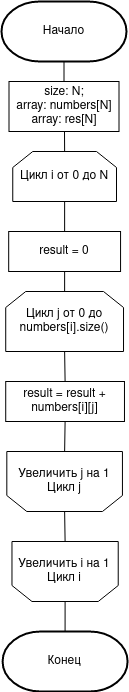
\includegraphics[width=.2\linewidth]{src/schemas/consistent.png}\\
	Рис. 2.1: Схема последовательного алгоритма подсчёта
\end{center}
\clearpage
На рисунке 2.2.1 представлена схема главного потока первого парллельного алгоритма.\\
\begin{center}	
	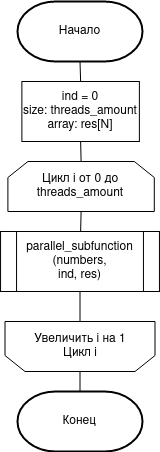
\includegraphics[width=.3\linewidth]{src/schemas/parallel1_main.png}\\
	Рис. 2.2.1: Схема главного потока первого парллельного алгоритма
\end{center}
\clearpage
На рисунке 2.2.2 представлена схема дочернего потока первого парллельного алгоритма.\\
\begin{center}	
	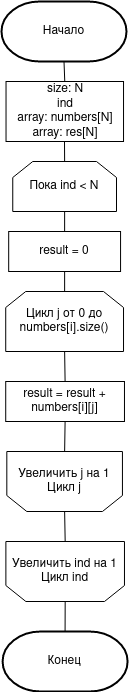
\includegraphics[width=.2\linewidth]{src/schemas/parallel1_thread.png}\\
	Рис. 2.2.2: Схема дочернего потока первого парллельного алгоритма
\end{center}
\clearpage
На рисунке 2.3.1 представлена схема главного потока второго парллельного алгоритма.\\
\begin{center}	
	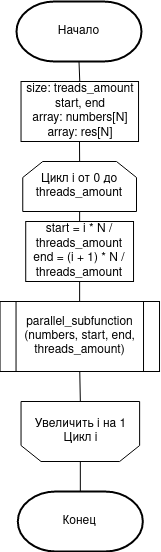
\includegraphics[width=.26\linewidth]{src/schemas/parallel2_main.png}\\
	Рис. 2.3.1: Схема главного потока второго парллельного алгоритма
\end{center}
\clearpage
На рисунке 2.3.2 представлена схема дочернего потока второго парллельного алгоритма.\\
\begin{center}	
	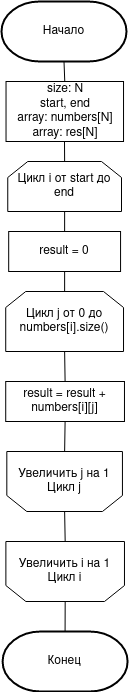
\includegraphics[width=.2\linewidth]{src/schemas/parallel2_thread.png}\\
	Рис. 2.3.2: Схема дочернего потока второго парллельного алгоритма
\end{center}
\clearpage
\addcontentsline{toc}{subsection}{Вывод}
\section*{Вывод}
\qquad В данном разделе были рассмотрены схемы реализуемых алгоритмов.
\clearpage

\section{Технологическая часть}
\qquad В данном разделе будет описана технологическая часть лабораторной работы: требования к ПО, листинг кода, сравнительный анализ всех алгоритмов.
\subsection{Требования к программному обеспечению}
\qquad Входные данные: размерность массива, сам массив\\
\qquad Выходные данные: массив с суммами элементов подмассивов\\
\qquad Среда выполнения: Linux Ubuntu 20.04 x64\\
\qquad CPU: Intel Core i7-8550U
\subsection{Средства реализации}
\qquad Для выполнения данной лабораторной работы использовался язык программирования C++ стандарта 2020 года, а также среда разработки CLion 2020.2. Для замены времени было использовано средство \textbf{std::chrono} \cite{litlink4}
\subsection{Листинг кода}
\qquad В данном разделе будет представлен листинг кода разработанных алгоритмов.\\

Ниже, на листинге 3.1, представлена реализация последовательного алгоритма подсчёта:
\begin{center}
	Листинг 3.1: Последовательный алгоритм подсчёта
	\lstinputlisting[language=C++]{src/code/consistent.cpp}
\end{center}
\clearpage

Ниже, на листинге 3.2.1, представлена реализация главного потока первого параллельного алгоритма подсчёта:
\begin{center}
	Листинг 3.2.1: Главный поток первого алгоритма подсчёта
	\lstinputlisting[language=C++]{src/code/parallel1_main.cpp}
\end{center}

Ниже, на листинге 3.2.2, представлена реализация дочернего потока первого параллельного алгоритма подсчёта:
\begin{center}
	Листинг 3.2.1: Дочерний поток первого алгоритма подсчёта
	\lstinputlisting[language=C++]{src/code/parallel1_thread.cpp}
\end{center}
\clearpage

Ниже, на листинге 3.3.1, представлена реализация главного потока второго параллельного алгоритма подсчёта:
\begin{center}
	Листинг 3.3.1: Главный поток второго алгоритма подсчёта
	\lstinputlisting[language=C++]{src/code/parallel2_main.cpp}
\end{center}

Ниже, на листинге 3.3.2, представлена реализация дочернего потока второго параллельного алгоритма подсчёта:
\begin{center}
	Листинг 3.3.2: Дочерний поток второго алгоритма подсчёта
	\lstinputlisting[language=C++]{src/code/parallel2_thread.cpp}
\end{center}
\clearpage


\subsection{Описание тестирования} % описать, какие тесты будут проведены ВСЕ ТЕСТЫ ПРОЙДЕНЫ УСПЕШНО
Были проведены тесты на больших размерностях со случайными строками в качестве элементов.\\
\qquad Ниже, на листинге 3.4, представлен фрагмент кода тестирования корректной работы реализации алгоритмов
\begin{center}
	Листинг 3.4: Тестирование корректной работы алгоритмов
	\lstinputlisting[language=C++]{src/code/tests.cpp}	
\end{center}

Все тесты пройдены успешно.

\addcontentsline{toc}{subsection}{Вывод}
\section*{Вывод}
\qquad В данном разделе был представлен листинг реализованных алгоритмов, а также описание тестирование корректности их работы.
\clearpage

\section{Экспериментальная часть}
\qquad В данной части работы будут приведен анализ алгоритмов на основе эксперементальных данных.
\subsection{Сравнительный анализ на основе замеров времени работы алгоритмов}
Для сравнения замеров времени были взяты подмассивы размерами по 1000 элементов и длины массивов от 10000 до 50000 с шагом 10000.
Каждый эксперимент на каждой размерности был произведён 10 раз, затем бралось среднее арифметическое полученного результата.
Ниже, на графике 4.1, видно, что обе параллельные версии алгоритма выигрывают у последовательной:\\
\begin{center}
	\begin{tikzpicture}
	\begin{axis}[
	axis lines = left,
	xlabel = {Количество подмассивов},
	ylabel = {Время (с)},
	legend pos=north west,
	ymajorgrids=true
	]
	\addplot[color=red, mark=square] table[x index=0, y index= 1] {src/graph/compare_consistent.txt}; 
	\addplot[color=green, mark=square] table[x index=0, y index= 1] {src/graph/compare_parallel1.txt}; 
	\addplot[color=blue, mark=square] table[x index=0, y index= 1] {src/graph/compare_parallel2.txt}; 
	
	\addlegendentry{Последовательный алгоритм}
	\addlegendentry{Первый параллельный алгоритм (16 потоков)}
	\addlegendentry{Второй параллельный алгоритм (16 потоков)}
	
	\end{axis}
	\end{tikzpicture}\\
	График 4.1: Замеры вермени работы алгоритмов\\
\end{center}
Был проведён замер времени работы каждого из параллельных алгоритмов. Длина каждого подмассива 10000 символов. Каждый эксперимент на каждой размерности был произведён 10 раз, затем бралось среднее арифметическое полученного результата.\\
Все эксперименты были проведены для 80000 подмассивов.\\
Ниже во всех таблицах время выполнения указано в секундах.\\

Ниже, на графике 4.2, показана зависимость времени выполнения программы от количества потоков для первой параллельной версии алгоритма:\\

\begin{center}
	\begin{tikzpicture}
	\begin{axis}[
	axis lines = left,
	xlabel = {Количество потоков},
	ylabel = {Время (с)},
	legend pos=north west,
	ymajorgrids=true
	]
	\addplot[color=red, mark=square] table[x index=0, y index= 1] {src/graph/parallel1_threads.txt};
	
	\end{axis}
	\end{tikzpicture}\\
	График 4.2: Замеры вермени работы первого параллельного алгоритма\\
\end{center}

Ниже, на графике 4.3, показана зависимость времени выполнения программы от количества строк и количества потоков для первой параллельной версии алгоритма:\\


\begin{center}
	\begin{tikzpicture}
	\begin{axis}[
	axis lines = left,
	xlabel = {Количество потоков},
	ylabel = {Время (с)},
	legend pos=north west,
	ymajorgrids=true
	]
	\addplot[color=red, mark=square] table[x index=0, y index= 1] {src/graph/parallel2_threads.txt}; 
	
	\end{axis}
	\end{tikzpicture}\\
	График 4.3: Замеры вермени работы второго параллельного алгоритма\\
\end{center}
В результате экспериментов было выяснено, что максимальной производительности в обоих реализация удалость достичь при использовании 16 потоков благодаря технология Intel® Hyper-Threading.\\

\section*{Вывод}
По результатам исследования получилось, что обе параллельные версии алгоритма
работают приблизительно за равное время, но каждая из них быстрее классического алгоритма. Также установлено, что увеличение количества потоков имеет смысл, пока не будет достигнуто число, равное количеству логических потоков в системе. Причем самой быстрой версией параллельного алгоритма(любой из его версий) является та, где число потоков равно числу логических процессоров.
Но если процессор поддерживает технологию Intel® Hyper-Threading, то программа наилучшим образом будет работать при количестве потоков, равному удвоенному количеству потоков в процессоре.
\clearpage

\addcontentsline{toc}{section}{Заключение}
\section*{\Huge Заключение}
\qquad В ходе работы были изучен алгоритм подсчета суммы каждого подмассива в массиве, а также разработаны 3 версии этого алгоритма: 1 последовательная и 2 параллельных. Экспериментально было установлено, что параллельные версии быстрее классического алгоритма, причем чем больше количество подмассивов на вход - тем больше выигрыш. Было
установлено, что максимальная скорость работы параллельных алгоритмов достигается при равенстве количества потоков числу логических процессоров в системе.

%//////////////////////////////////////////////////////////////////
\clearpage
\begin{thebibliography}{}
	\bibitem{litlink1} Справка по потокам в ОС Windows // https://docs.microsoft.com/en-us/windows/win32/procthread/process-and-thread-functions (дата обращения: 27.10.2020).
	\bibitem{litlink2} Кнут Д. Э. Искусство программирования. Том 1. Сортировка и поиск . -- М.: Вильямс, 2007. -- 832 с.
	\bibitem{litlink3} Богачев К.Ю Основы параллельного программирования. -- М.: БИНОМ. Лаборатория знаний 2003.  -- 237 с.
	\bibitem{litlink4} Справка по C++ // cppreference URL: https://en.cppreference.com/w/ (дата обращения: 27.10.2020).
\end{thebibliography}
\end{document}